% Dokumentation af converter topologi

\chapter{Switch-Mode Power Supply}
%TODO Skriv hvorfor der er valgt SMPS frem for lineær forsyning

\section{Flyback Converter}
Flyback converteren, er en transformator baseret topologi. Man deler converteren op i to dele: Primær- og sekundærsiden. Primærsiden består af en transistor, forbundet i serie med primærviklingen af transformatoren, hvor transistoren fungerer som en switch. Sekundærsiden består af en parallelforbindelse mellem sekundærviklingen og en diode i serie, en udgangskondesator, samt belastningen. Dette er også vist på figur~\ref{fig:flyback_ideal}. En af fordelene ved at bruge flyback converteren er at der kan opnås galvanisk adskillelse mellem primær- og sekundærsiden af transformatoren. 

\begin{figure}[H]
	\center
	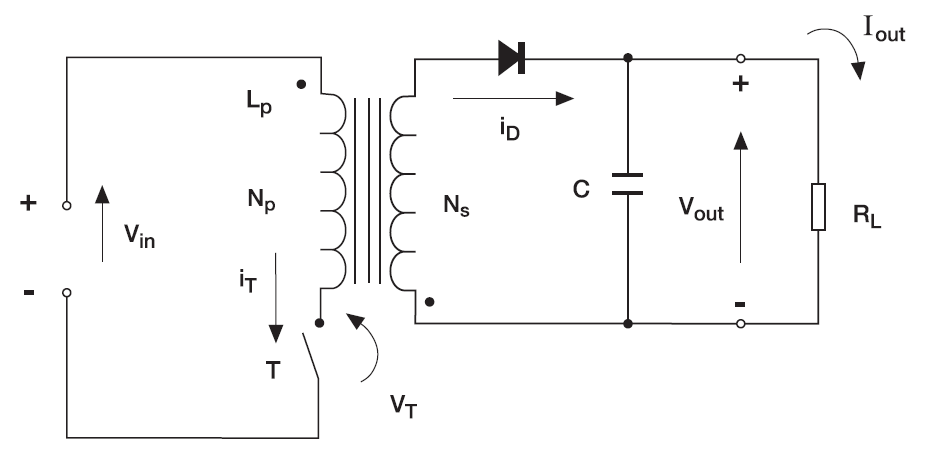
\includegraphics[max width=0.7\linewidth]{/tex/smps/billeder/flyback_ideal.PNG}
	\caption{Ideelt diagram af flyback converteren
	\cite{SMPS-topologies}}
	\label{fig:flyback_ideal}
\end{figure} 

\noindent Flyback converteren bruges til at konvertere en indgangsspænding, ned til en mindre udgangsspænding. Dette gøres ved at styre transistoren med digitalt signal, med en variabel duty-cycle. Når transistoren er ON, vil der være en positiv spænding ved prik-enden af viklingen ift. den anden ende. Ud fra formlen $V=L\cdot \frac{di}{dt}$ kan det ses, at når der ligger en spænding over viklingen, vil strømmen i transformatoren stige lineært, over den tid transistoren er ON. Når transistoren går OFF, vil den magnetiske strøm i transformatoren inducere en spænding over sekundærviklingen. Nå denne spænding bliver lig udgangsspændingen, vil dioden begynde at lede den strøm, der er oplagret i transformatoren. Da spændingen over sekundærviklingen er positiv ved prikken, og dermed modsat af primærviklingen, vil strømmen falde lineært ud fra samme forhold, som nævnt tidligere. Dette vil over tid skabe en trekantet kurveform af den samlede strøm i transformatoren. Et eksempel på dette kan ses på figur \ref{fig:CCM_transformer_current}.

Udgangskondensatoren har to funktionaliteter. Den skal kunne holde spændingen over belastningen i transistorens ON periode. Derudover er den, sammen med sekundærviklingen af transformatoren, en del af et 2. ordensfilter, som minimerer ripplespændingen på udgangen.

Flyback converteren kan overordnet drives på to forskellige måder, Continuous Conduction Mode (CCM) og Discontinuous Conduction Mode (DCM). Disse to måder har forskellige fordele og ulemper, som skal tages højde for inden der vælges hvordan converteren skal drives. 

\subsection{Continuous Conduction Mode}
Forkellen ved CCM og DCM er, hvordan strømmen løber i transformatoren. Ved CCM vil der altid løbe en strøm i transformatoren, som der også ligger i navnet. Strømmen er skitseret på figur \ref{fig:CCM_transformer_current}. Skal man have den samlede strøm i transformatoren, skal de to kurver for primær- og sekundærviklingen samles. Dette er fordi der kun løber en strøm i primærviklingen når transistoren er ON, og en strøm i sekundærviklingen når transistoren er OFF. 

\begin{figure}[H]
	\center
	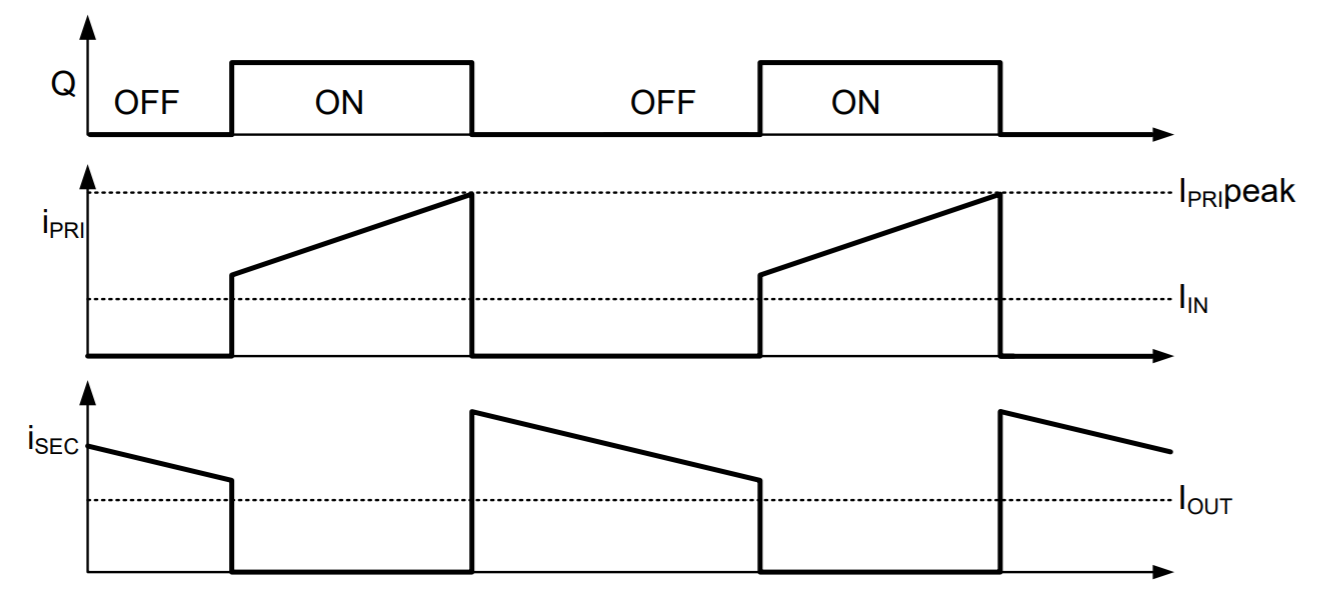
\includegraphics[max width=0.7\linewidth]{/tex/smps/billeder/CCM_transformer_current.PNG}
	\caption{CCM transformator strømme}
	%\cite{SMPS-topologies}}
	\label{fig:CCM_transformer_current}
\end{figure}

\noindent En af fordelene ved CCM er, at strømmen i transformatoren ikke når at aflade helt, inden transistoren går ON igen. Dette giver lavere peak-strømme, som sætter mindre krav til transistor og diode, og giver anledning til et mindre tab. Da transformatoren ikke når at aflade får man også en mindre ripplestrøm i transformatoren, $\Delta i$, og dermed også en mindre ripplespænding på udgangen. 

\subsection{Discontinuous Conduction Mode}

